\esSezione{Sistema ROM + M}\label{sec:esercizio2-1}

\begin{traccia}
Progettare, implementare in VHDL e testare mediante simulazione un sistema $S$ composto da una ROM puramente combinatoria di 16 locazioni da 8 bit e da una macchina combinatoria $M$. Fornito un indirizzo $A$ di 4 bit, il sistema restituisce il contenuto della ROM all'indirizzo $A$ trasformato da $M$. Il comportamento di $M$ è a scelta, con il solo vincolo di 8 bit in ingresso e 4 bit in uscita.
\end{traccia}

\progetto

Il sistema è formato da due componenti collegati in cascata: la ROM, che riceve l'indirizzo a 4 bit e fornisce il dato a 8 bit, e la macchina combinatoria $M$, che riduce tale dato a 4 bit. Il sistema è puramente combinatorio, senza clock né reset. Come funzione di $M$ è stata scelta l'AND tra coppie di bit adiacenti del dato letto: ciascuno dei quattro bit di uscita è l'AND di due bit consecutivi dell'ingresso.

Il top module \texttt{systemS} istanzia i due componenti e li collega tramite un segnale interno a 8 bit. Rispetto alla soluzione proposta, l'implementazione usa nomi diversi (\texttt{rom16\_8}, \texttt{systemM}, \texttt{systemS}) e istanzia i componenti in modo diretto (\texttt{entity work.\ldots}) anziché con dichiarazione di \texttt{component}. La struttura del sistema è riassunta in figura~\ref{fig:esercizio2-1:schema}.

\begin{figure}[H]
  \centering
  \begin{tikzpicture}[node distance=2.2cm]
    \node[blocco, minimum width=2.6cm, minimum height=1.4cm] (rom) {\texttt{rom16\_8}\\ (\texttt{MEM})};
    \node[blocco, minimum width=2.6cm, minimum height=1.4cm, right=of rom] (m) {\texttt{systemM}\\ (\texttt{SYSTEM\_M})};
    \node[draw, dashed, thick, inner xsep=0.6cm, inner ysep=0.5cm, fit=(rom)(m), label={[font=\sffamily\small]above:\texttt{systemS}}] (s) {};
    \draw[bus] ($(s.west |- rom)+(-2.4,0)$) -- node[pos=0.2, above=3pt, font=\scriptsize] {\texttt{input}} node[pos=0.5, sloped, inner sep=1pt]{/} node[pos=0.5, below=3pt, font=\scriptsize]{4} (rom.west);
    \draw[bus] (rom) -- node[pos=0.5, sloped, inner sep=1pt]{/} node[pos=0.5, below=3pt, font=\scriptsize]{8} node[pos=0.5, above=3pt, font=\scriptsize] {\texttt{q}} (m);
    \draw[bus] (m.east) -- node[pos=0.5, sloped, inner sep=1pt]{/} node[pos=0.5, below=3pt, font=\scriptsize]{4} node[pos=0.88, above=3pt, font=\scriptsize] {\texttt{output}} ($(s.east |- m)+(2.4,0)$);
  \end{tikzpicture}
  \caption{Schema a blocchi del sistema ROM + M}
  \label{fig:esercizio2-1:schema}
\end{figure}

\implementazione

L'entità \texttt{rom16\_8} ha come ingresso \texttt{address} (4 bit) e come uscita \texttt{data} (8 bit). Nell'architettura \texttt{Behavioral} si trova un array di 16 elementi da 8 bit, inizializzato con valori esadecimali, e un process, sensibile ad \texttt{address}, assegna a \texttt{data} l'elemento indicato dall'indirizzo convertito in intero. L'attributo \texttt{rom\_style} è impostato a \texttt{"block"}. Il contenuto della ROM (da 0x4A a 0xED) differisce da quello della soluzione proposta (0xA8, 0xBD, \ldots), che ripete due volte la stessa serie di otto valori.

\vhdlfile{esercizio2-1/rom16_8.vhd}{Implementazione ROM 16x8}{lst:esercizio2-1:rom16-8}

L'entità \texttt{systemM} ha l'ingresso \texttt{data\_in} (8 bit) e l'uscita \texttt{data\_out} (4 bit). L'architettura \texttt{dataflow} assegna a ciascun bit di uscita l'AND di due bit adiacenti: \texttt{data\_out(0)} da \texttt{data\_in(0)} e \texttt{data\_in(1)}, \texttt{data\_out(1)} da \texttt{data\_in(2)} e \texttt{data\_in(3)}, e così via fino a \texttt{data\_out(3)}. A differenza della soluzione proposta, le porte sono dichiarate con indici decrescenti (\texttt{7 downto 0}).

\vhdlfile{esercizio2-1/systemm.vhd}{Implementazione macchina combinatoria M}{lst:esercizio2-1:systemm}

Definite le due entità, il top module \texttt{systemS} ha l'ingresso \texttt{input} e l'uscita \texttt{output}, entrambi a 4 bit. L'architettura \texttt{structural} dichiara il segnale \texttt{q}, a 8 bit, che porta il dato dalla ROM a $M$, e istanzia \texttt{rom16\_8} (etichetta \texttt{MEM}) e \texttt{systemM} (etichetta \texttt{SYSTEM\_M}) con port mapping per nome.

\vhdlfile{esercizio2-1/systems.vhd}{Implementazione del sistema ROM + M}{lst:esercizio2-1:systems}

\simulazione

Il testbench \texttt{systemS\_tb} ha entità senza porte. Istanzia il sistema sotto test (\texttt{SYSTEM\_S}) e una seconda istanza di \texttt{systemM}, usata come riferimento, alimentata con i valori di una copia della ROM (\texttt{ref\_mem}) dichiarata nel testbench. Il process \texttt{stim\_proc} attende \SI{10}{ns}, poi con un ciclo \texttt{for} da 0 a 15 applica l'indirizzo \texttt{x} e carica in \texttt{ref\_in} il dato corrispondente. Dopo \SI{10}{ns} confronta \texttt{y} con \texttt{ref\_out} tramite \texttt{assert}, con \texttt{severity failure} in caso di differenza, e termina con \texttt{wait;}.

\vhdlfile{esercizio2-1/systems_tb.vhd}{Testbench sistema ROM + M}{lst:esercizio2-1:systems-tb}

Il risultato della simulazione è mostrato in figura~\ref{fig:esercizio2-1:simulazione}.

\begin{figure}[H]
  \centering
  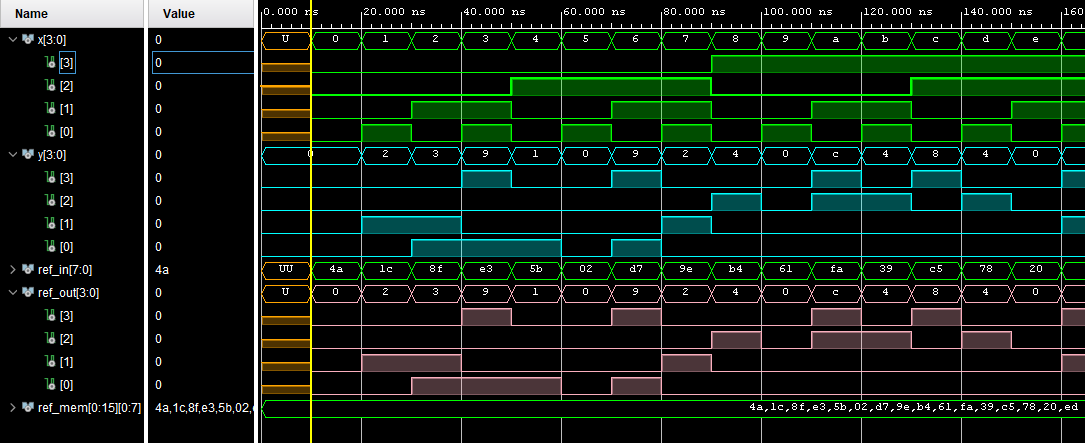
\includegraphics[width=0.95\linewidth]{figure/esercizio2-1/simulazione}
  \caption{Simulazione sistema ROM + M}
  \label{fig:esercizio2-1:simulazione}
\end{figure}

Per l'indirizzo \texttt{x} $= 1$ ($0001_2$) il sistema legge dalla ROM il valore 0x1C ($00011100_2$), presente in \texttt{ref\_in}. Le coppie di bit adiacenti, dalla meno significativa, valgono $00$, $11$, $01$, $00$: l'uscita \texttt{y} è quindi $0010_2$, cioè 2 in esadecimale, uguale a \texttt{ref\_out}. Lo stesso vale per tutti i sedici indirizzi e l'\texttt{assert} non segnala errori.

\begin{risultato}
Per i sedici indirizzi, \texttt{y} coincide con \texttt{ref\_out} (ad esempio 0x2 per l'indirizzo 1 e 0x3 per l'indirizzo 2).
\end{risultato}
